%!TEX root = thesis.tex

\chapter{Gesture recognition}
\label{ch:gestures}



\section{Feature extraction}

\subsection*{Segmentation - removing background}

\begin{figure}[htbp]
\begin{center}
\subfloat[Hand window]{
        
\includegraphics[width=0.2\linewidth]{figures/pipeline/lefthand.jpg}
        \label{fig:lefthandwindow}
}
\hspace{0.03\linewidth}
\subfloat[Hand cutout]{
        
\includegraphics[width=0.2\linewidth]{figures/pipeline/lefthandcutout.jpg}
        \label{fig:lefthandcutout}
}
\hspace{0.03\linewidth}
\subfloat[Hand features]{
        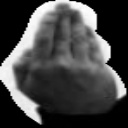
\includegraphics[width=0.2\linewidth]{figures/pipeline/lefthandhog.jpg}
        \label{fig:lefthandfeatures}
}
\end{center}
\end{figure}

A cutout of a hand from a image still contains some background pixels, because a hand will never fill a perfect square. These pixels are unwanted since they contain arbitrary values that introduce noise into our process. In section \ref{sec:skinmodel} a binary mask for skin pixels is constructed. The binary inversion of this mask can be used again to remove the background. The result of this procedure can be seen in figure \ref{fig:gijs5_cutout}. To decrease the possibility that mislabeled skin pixels are removed by this mask, a small morphological dilate operation will increase the size of the hand cutout, but this will also introduce more noisy (background) pixels.


\subsection*{Histogram of Oriented Gradients}
Histogram of oriented gradient (HOG) descriptors are feature descriptors used for object detection. It has been successfully applied and studied in human detection \cite{NavneetDalal2006}.  The HOG descriptors method is similar to that of edge orientation histograms, scale-invariant feature transform descriptors, and shape contexts, but differs in that it uses a dense grid of uniformly spaced cells and uses overlapping local contrast normalization for improved accuracy.

For the experiments described in chapter \ref{ch:experiments} the same parameters as in the \cite{watanabe2009} paper are used, except that the image is not resized to 64 by 128 pixels, but 128 by 128 pixels.

hand detection with SIFT\cite{Wang2007}

\section{Classification}

\subsection*{Classifier}
Two classifiers where evaluation during the experiments, K-Nearest Neighbors (KNN) and Support Vector Machines (SVM). For the experiments with KNN different values for $k$ where evaluated. The experiments with SVM where more profound, different kernels and parameters where evaluated. The evaluated kernels are the Radial Basis Function (RBF) and a precomputed kernel using the $\chi^2$ method on the train set. For the RBF kernel 2 parameters are important, the cost $c$ and $\gamma$. The optimal values of these variables for these experiments where found with a brute force grid search on a small cluster.

Also Principal Component Analysis (PCA) was performed on the dataset to reduce the dimensionality. The impact on the classifiers has been measured and is presented together with all other experiments in chapter \ref{ch:experiments}.

\subsection*{The stabilizer}
Since the frames following each other have a spatio-temporal relationship there is a relationship between the labels given by the classifier. Because of noise, misclassification can happen. These false matches can be filtered out by smoothing the labels on a time scale.

This smoothing is done with a simple self invented method called 'the stabilizer'. 

The stabilizer is initialized with $n$ numbers of bins which is equal to the number of labels. There are 2 parameters, $n_{max}$ and $n_{threshold}$.

For every new label that is given by the classifier all bins are decremented with 1, except for the bin with the currently classified label which is incremented. A bin is incremented until it reaches it maximum value. When at any moment one of the bins value rises above the threshold, the stabilizer will output the label of that bin, as if it was the classifier itself. The result is a more stable and smoothed stream of labels, where single noisy labels are filtered out. For a sequence of frames with a correctly detected pose there is a delay between the first frame and the stabilizer will output the correct label, this delay is controlled by $n_{threshold}$ which is measured in frame count. A higher value will reduce more noise, but will give a bigger delay. There is also a delay after a sequence which is controlled by $n_{max}$. With a framerate of $25$ frames a second, $n_{max} = 15$ and $n_{threshold} = 10$ give good results reducing noise and still being very responsive. 

\subsection*{Training phase}
recording video, manual labeling, extracting HOG features, training classifier

\section{Discussion}
